% This text is proprietary.
% It's a part of presentation made by myself.
% It may not used commercial.
% The noncommercial use such as private and study is free
% Dec 2007
% Author: Sascha Frank 
% University Freiburg 
% www.informatik.uni-freiburg.de/~frank/
%
% 
\documentclass{beamer}
\setbeamertemplate{navigation symbols}{}
\usetheme{Warsaw}

\usepackage[export]{adjustbox}

\usepackage[thinlines]{easytable}

\beamersetuncovermixins{\opaqueness<1>{25}}{\opaqueness<2->{15}}

\def\mydot{\structure{\rule{1ex}{1ex}}\,}
\def\B#1{\mathbf{#1}}
\def\emph#1{\textbf{\textcolor{orange}{#1}}}
\def\photocredit#1{\vspace{-.5em}{\tiny \textit{(Picture is courtesy of #1)}}}
\def\leadto{$\mathbf{\implies}$}
\DeclareMathOperator{\argmin}{argmin}
\DeclareMathOperator{\prox}{prox}
\DeclareMathOperator{\proj}{proj}

\newcommand{\mycite}[1]{\textcolor{myblue}{\text{ [#1]}}}

%% put page number in slide footer
\newcommand*\oldmacro{}%
\let\oldmacro\insertshorttitle%
\renewcommand*\insertshorttitle{%
  \oldmacro\hfill%
  \insertframenumber\,/\,\inserttotalframenumber}

\definecolor{darkgreen}{rgb}{0,0.5,0}
\definecolor{myblue}{RGB}{102,153,255}
\definecolor{mygray}{RGB}{200,200,200}

\AtBeginSection[]{
  \begin{frame}
  \vfill
  \centering
  \begin{beamercolorbox}[sep=8pt,center,shadow=true,rounded=false]{title}
    \usebeamerfont{title}\insertsectionhead\par%
  \end{beamercolorbox}
  \vfill
  \end{frame}
}

\begin{document}

\section{Appendix}
\begin{frame}
  \frametitle{{Tuning SODL model hyper-parameters}}%\Large
  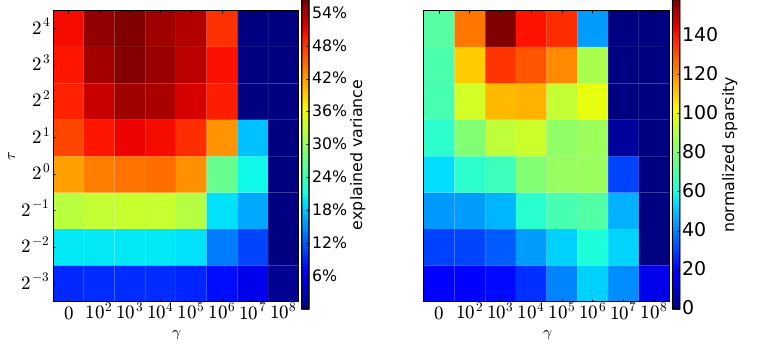
\includegraphics[width=1.\linewidth]{cv.png}
  \bigskip
  
  \mydot{The red spots are the best spots}

  \bigskip
  
  \mydot{Can be located find them via cross-validation}
\end{frame}

\begin{frame}\frametitle{How fMRI data is acquired}
    \centering
    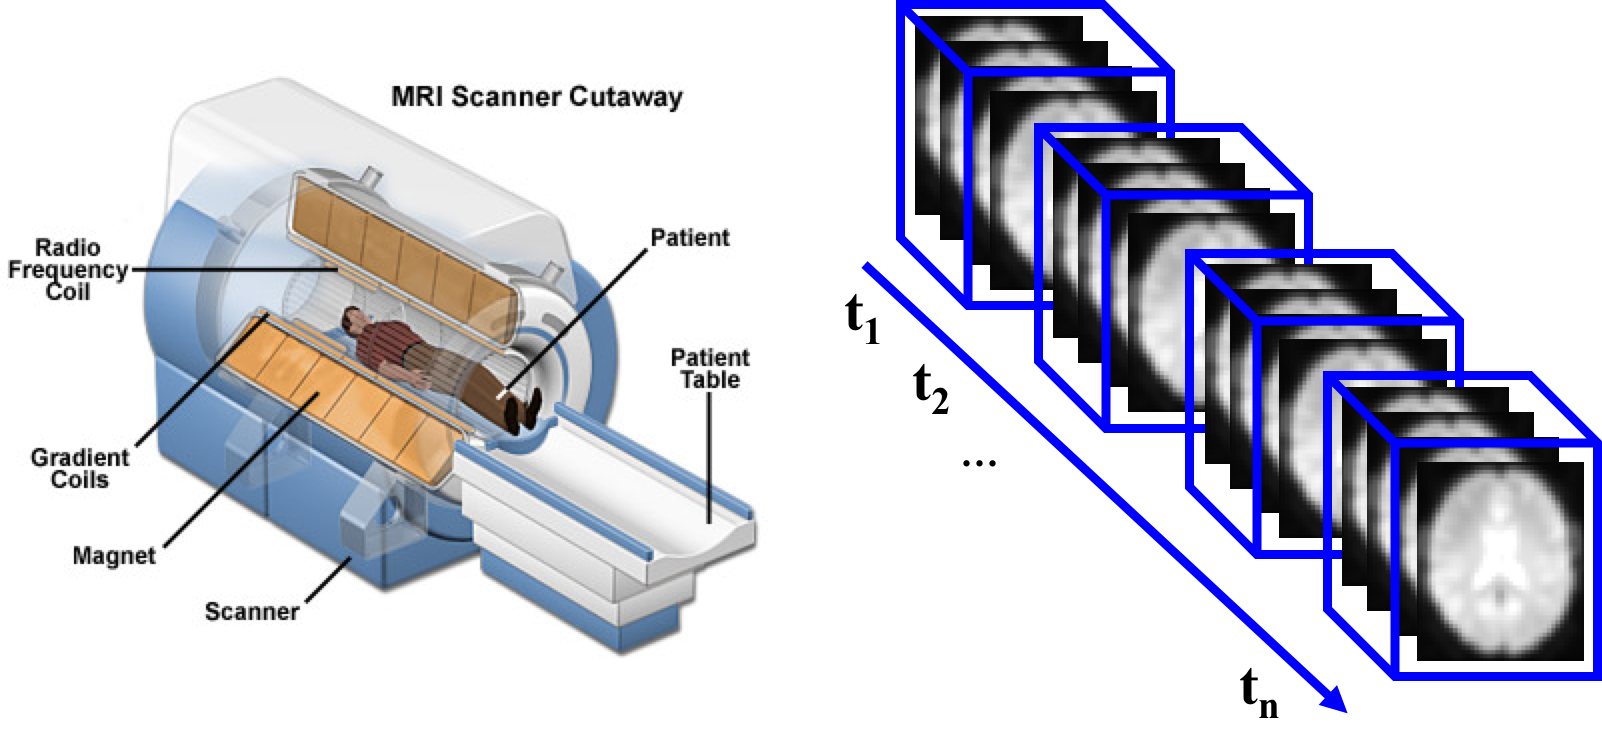
\includegraphics[scale=.4]{fmri_setup}

\tiny{\textit{(Courtesy of ???)}}
\end{frame}

\subsection{Proximal online updates for dictionary-learning}
\begin{frame}
  \frametitle{Ongoing work: proximal online updates }
  \vspace{-2em}
\begin{table}[H]
  \begin{tabular}{p{3.cm}|c|p{13cm}}\hline
    \emph{penalty $g$} & \emph{$\B{p} = \prox_{\gamma g}(\B{z})$} & \emph{comments}\\\hline
    L2 ball constraint & $p_v = \B{z}_v\frac{\gamma}{\max(\gamma,\|\B{z}\|_2)}$ & \mycite{Mairal 2010}\\ \hline
%    nonneg. constraint & $p_v = (\B{z}_v)_+$ & used in NMF\\ \hline
    convex constraint & $\B{p} = \proj_{\mathcal K}(\B{z})$ & interesting for simple $\mathcal K$\\ \hline
    L1 penalty & $p_v = z_v\left(1 - \frac{\alpha}{|z_v|}\right)_+$ & soft-thresholding \\\hline
    Group L2/L1 & $\B{p}_v = \B{z}_v\left(1 - \frac{\gamma}{\|\B{z}_v\|_2}\right)_+$ & $i$ is a group of features\\\hline
    Social sparsity \newline \mycite{Kowalski '09} & $p_v = z_v\left(1 - \frac{\gamma}{\|\boldsymbol{\omega}_v * \B{z}\|_2}\right)_+$
                                                    & feature $i$ survives if avg. \newline energy in neigh. is high\\\hline
    % Social sparsity & $p_v = z_v\left(1 - \frac{\gamma}{\left(\sum_{l \in \mathcal N(i)}(\omega^{l}_{i})^2z_{l}^2\right)^{1/2}}\right)_+$
    %                                                 & denominator is just a \newline
    %                                                 convolution\\\hline
%    etc. & etc. & etc.\\\hline
  \end{tabular}
\end{table}

\vspace{-1.5em}
\begin{overlayarea}{\textwidth}{\textheight}
\begin{columns}
  \column{.35\linewidth}
  \only<2->{
    \vspace{3.5em}
    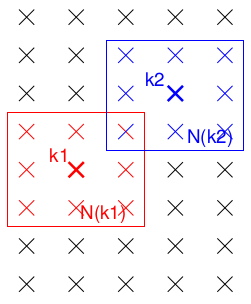
\includegraphics[width=.8\linewidth]{social.png}
  }

\vspace{-4em}  
\column{.65\linewidth}
\only<3->{
  \emph{Zoom on social sparsity }\mycite{Kowalski '09}

  \mydot $\|\boldsymbol{\omega}_v * \B{z}\|_2^2 := \sum_{l \in \mathcal N(i)}\omega^{l}_{i}z_{l}^2 \ge 0$%, a convolution with weights $\omega_v^1, \ldots,\omega_v^p \ge 0$,
%  where $\sum_{i}\omega_v^l = 1$, $\forall l \in [\![p]\!]$

  \bigskip
  
  \mydot Imposes \emph{sparsity} and \emph{smoothness}!
  }
\end{columns}
\end{overlayarea}
\end{frame}

\begin{frame}
  \frametitle{{proximal online updates }}
  % \mydot Our proposed model can an be extended to more general structured penalties of the form \emph{$\Omega(\B{D}) := \sum_{j=1}^kg_j(\B{d}^j)$}. Viz,
  \mydot \emph{N.B.:}  Ongoing work
  
  \begin{overprint}
    \onslide<1>
    \begin{eqnarray*}
      \begin{split}
        &\min_{\B{D} \in \mathbb R^{p \times k}}\frac{1}{n}\sum_{t=1}^n\left(\min_{\B{c}_t \in \mathbb R^{k}}\frac{1}{2} \|\B{x}_t-\B{D}\B{c}_t\|_2^2 +  \alpha\|\B{c}_t\|_2^2\right) + \gamma\textcolor{red}{\sum_{j=1}^k\Omega_{\text{Lap}}(\B{d}^j)}.\\
    &\textcolor{red}{\text{subject to } \B{d}^1,\ldots,\B{d}^k \in \mathcal K}
  \end{split}
    \end{eqnarray*}
\onslide<2->
\begin{eqnarray*}
  \begin{split}
&\min_{\B{D} \in \mathbb R^{p \times k}}\frac{1}{n}\sum_{t=1}^n\left(\min_{\B{c}_t \in \mathbb R^{k}}\frac{1}{2} \|\B{x}_t-\B{D}\B{c}_t\|_2^2 +  \alpha\|\B{c}_t\|_2^2\right)
     + \gamma\textcolor{green}{\sum_{j=1}^kg_j(\B{d}^j)}.
   \end{split}
\end{eqnarray*}
\end{overprint}

% \mydot Here, the \emph{$g_j$}'s are \textit{proximable} (e.g group-Lasso, social sparsity)
% \bigskip
\uncover<3->{
\textbf{\textcolor{orange}{The proximal online BCD updates:}}\\
\begin{equation*}
  \begin{split}
    \vspace*{-1em}
    \rlap{\smash{
\includegraphics[width=2em]{loop}}}%      
    \quad\quad\B{d}^j \leftarrow \prox_{\gamma a_{j,j}^{-1}g_j}(\B{z}^{-j}),\;j \leftarrow j + 1 \text{ (go to next atom)}
  \end{split}
  \end{equation*}
\mydot $\B{z}^{-j} := a_{j,j}^{-1}\B{r}^j$ and $\B{R} := \left(\B{b}^j-\sum\nolimits_{l \ne j}a_{j,l}\B{d}^l\right) = \B{B}- \B{DA} + \B{d}^j \circ \B{a}^j $.
}

\uncover<4->
{
  \mydot \emph{Bonus:} It suffices to specify the $g_j$'s only via their prox!
\begin{itemize}
\item E.g Social sparsity! \mycite{Kowalski '09}
\end{itemize}
}

\end{frame}


\begin{frame}\frametitle{Masking}
  \begin{columns}
    \column{.65\linewidth}
    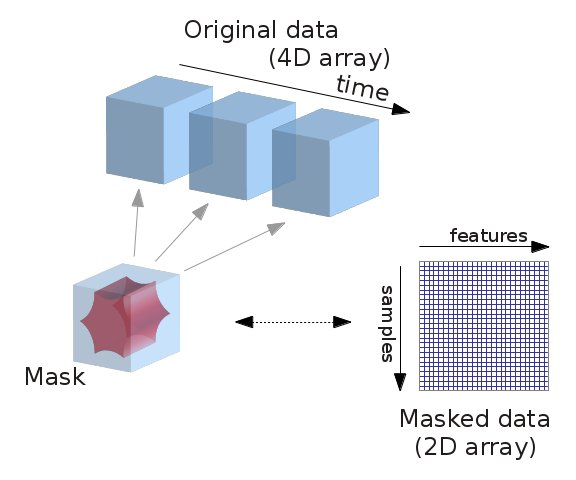
\includegraphics[width=1\linewidth]{masking.jpg}
    
    \photocredit{Alexandre Abraham}
    \column{.5\linewidth}
    \mydot time or sequence of subjects

    \bigskip
   
    \mydot 3D image $\iff$ vector in $\mathbb R^p$% (via mask).

    \bigskip
    
    \mydot Masking destroys spatial struct.
      \vspace{-1.5em}
      \begin{itemize}
      \item How to keep it ?
      \end{itemize}

    \bigskip
      
    \mydot It is all about matrices
  \end{columns}
\end{frame}

\end{document}